\section{问题一建模与求解}

为分析玻璃文物的表面风化与其玻璃类型、纹饰和颜色的关系以及文物样品表面有无风化化学成分含量的统计规律,并对风化前的化学含量进行分析,制作流程图如下:

\begin{figure}[H] 
	\centering %图片居中
	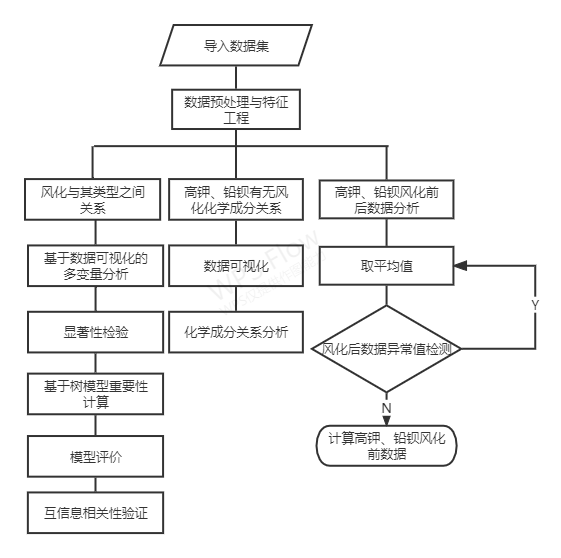
\includegraphics[width=0.7\textwidth]{1.png} %插入图片,[]中设置图片大小,{}中是图片文件名
	\caption{问题一流程图} %最终文档中希望显示的图片标题
	\label{Fig.main2} %用于文内引用的标签
\end{figure}

\subsection{模型准备——数据预处理与特征工程}

\subsubsection{数据清洗}

本文根据附件表1所给的数据,通过Pandas库进行数据读取,使用isnull函数查找数据中的缺失值,由此发现颜色特征中有数个缺失值,由数据可视化发现黑色文物必定被风化,而缺失值所在样本均为被风化对象,故采用黑色来补全缺失值。

对于附件表2所给的数据,表中空白部分为未检测到的成分将被Pandas视为缺失值,本文指定数值0填补空缺的值以避免缺失值对分析的干扰。

按照题意对其每一行进行求和,选取成分累加和介于85\% ~ 105\%的有效数据并删除不在有效数据范围内的第15个和第17个样品采样点的样本构成新的数据集用于分析。

\subsubsection{特征编码}

为更准确的判断风化情况与三个变量相关关系,依据表1所给的纹饰、类型、颜色以及表面是否风化四个特征对其用特征编码进行分类,由于各个类别之间是相互独立的,故采用独热编码进行特征变换以消除编码后各个类别的不同取值差异对模型训练效果的影响。

然而事与愿违,颜色特征中有七个非序数类别,而独热编码最大的缺点即容易造成编码后数据集的“高维危机”,由此针对颜色特征本文放弃了进行独热编码,而是对其特征编码。

\subsection{玻璃风化与其分类信息关系的分析模型}

\subsubsection{基于数据可视化的多变量分析}

本问要求分析玻璃纹饰、类型、颜色与表面风化情况的关系,基于多变量分析的数据可视化容易分别得到这三个分类特征与风化情况之间的关系,通过Pandas库中的crosstab函数可以实现分类特征之间的多变量分析,图形呈现如下:

\begin{figure}[H] 
	\centering %图片居中
	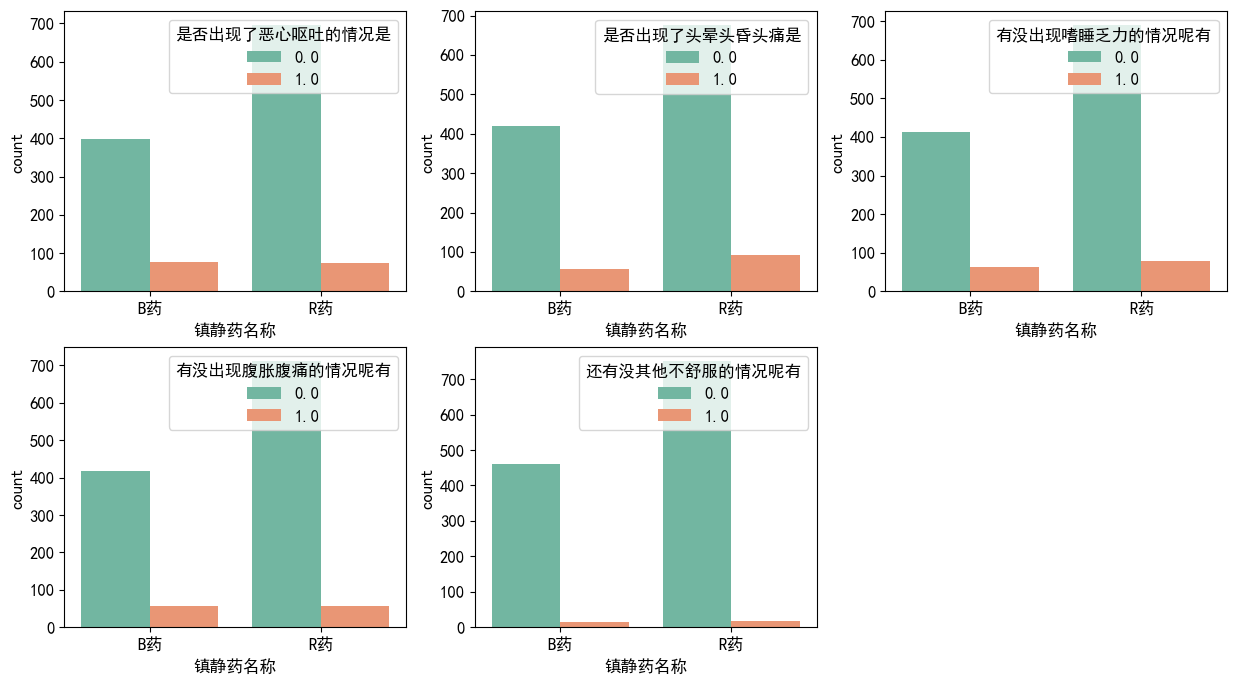
\includegraphics[width=0.7\textwidth]{2.png} %插入图片,[]中设置图片大小,{}中是图片文件名
	\caption{玻璃纹饰与风化情况关系} %最终文档中希望显示的图片标题
	\label{Fig.main3} %用于文内引用的标签
\end{figure}

由图2可知所提供的文物样品中A种纹饰的玻璃中近一半被风化,C种纹饰中风化的玻璃超过一半,而B种纹饰的玻璃全部风化——由此可以推断B类的纹饰与风化情况有极大联系。
下面再来考察玻璃类型与风化情况的关系:

\begin{figure}[H] 
	\centering %图片居中
	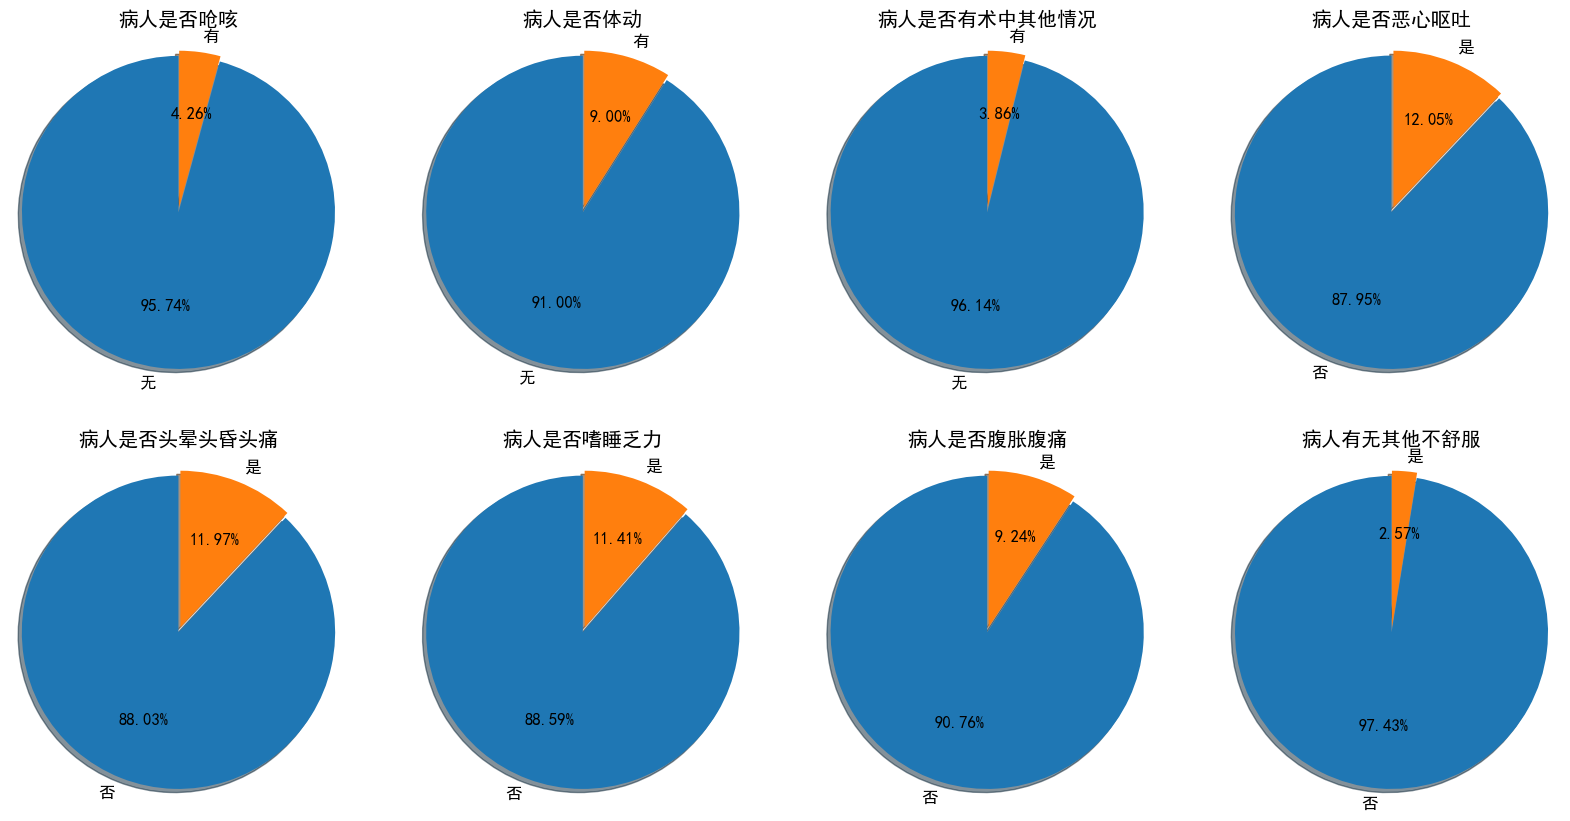
\includegraphics[width=0.7\textwidth]{3.png} %插入图片,[]中设置图片大小,{}中是图片文件名
	\caption{玻璃类型与风化情况关系} %最终文档中希望显示的图片标题
	\label{Fig.main4} %用于文内引用的标签
\end{figure}

由图3可知,对于样本所给的玻璃类型中高钾类玻璃风化的情况仅占百分之三十五,说明高钾类玻璃被风化的概率较小,而对于铅钡类的玻璃则是达到了百分之七十的风化比例。由此可见铅钡类玻璃更容易被风化。

\begin{figure}[H] 
	\centering %图片居中
	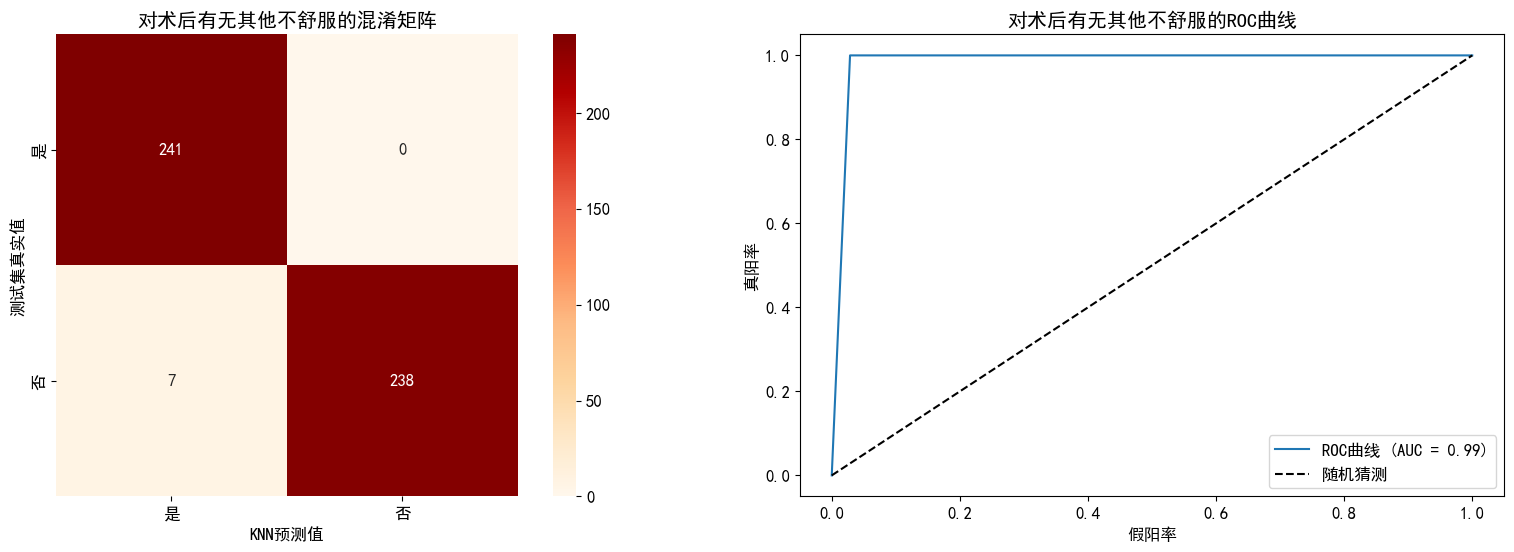
\includegraphics[width=0.7\textwidth]{4.png} %插入图片,[]中设置图片大小,{}中是图片文件名
	\caption{玻璃颜色与风化情况关系} %最终文档中希望显示的图片标题
	\label{Fig.main5} %用于文内引用的标签
\end{figure}

由图4可得,黑色的玻璃样本表面均被风化,而绿色和深蓝色的玻璃样本表面均为未被风化,其余颜色的样本表面被部分风化——由此可见黑色、绿色和深蓝色的玻璃与风化情况存在很大的关系,其他特征无法确定。

综上所述,可以总结出以下规律:

单个分类变量中玻璃纹饰和颜色都存在与表面风化情况确切相关的特征(如B种纹饰必定被风化,黑色文物必定风化,而深蓝和绿色文物均未被风化),而玻璃类型只能得到与风化情况的不同的频率,但不能确定是否风化,因此可以确定纹饰与颜色对玻璃风化的关系紧密,而玻璃类型可能相关性较弱。

下面通过集成学习中的树模型直接说明三种分类变量与玻璃风化情况的强弱关系。

\subsubsection{基于树的模型重要性计算}

通过模型准备中的特征工程本文已经实现了对数据分类特征的编码,经过模型准备的数据可以正式代入随机森林模型进行训练。

树模型作为一种集成学习算法,是一种效果优良的机器学习模型,且其独特的计算特征重要性的功能对于探索本问中多个变量的相关关系具用重要意义。本文基于树模型中最简单的Bagging算法——随机森林,对纹饰、类型、颜色与表面风化情况之间的关系进行分析,具体方法如下:

1. 为消除各类别之间的影响,便于对指标进行比较分析把分类特征编码数据标准化:进行标准化处理

\begin{equation}
  {{z}_{i}}=\frac{{{x}_{i}}-\overline{{{x}_{i}}}}{{{\sigma }_{i}}}
\end{equation}


2. 为找到最优模型,必须对树模型内部参数进行调整,找到最优参数,下面对最优参数进行探究。

(1)训练集的占比直接关系到模型的优劣,寻找训练集与测试集的占比最优参数,让模型达到较好的效果,利用scikit-learn库中的learning curve函数进行训练,并做交叉验证取平均值得到学习曲线图像如下:

\begin{figure}[H] 
	\centering %图片居中
	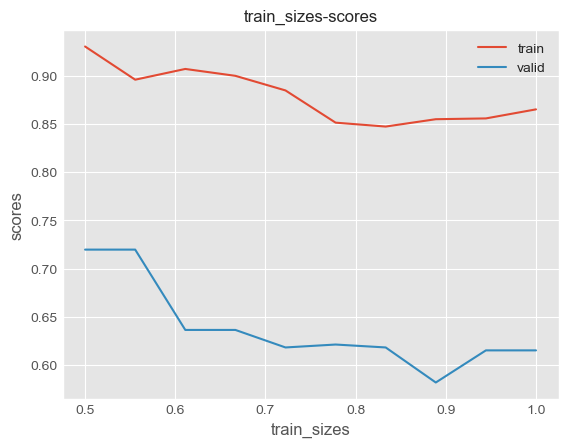
\includegraphics[width=0.7\textwidth]{5.png} %插入图片,[]中设置图片大小,{}中是图片文件名
	\caption{学习曲线} %最终文档中希望显示的图片标题
	\label{Fig.main6} %用于文内引用的标签
\end{figure}


图5可知,训练集占比0.5时,测试集效果最好,因此设置训练集占比为0.55是为最优训练集占比参数。

(2)对于树模型而言,大多数情况下其基学习器的数量是影响其性能的最重要的参数。通过GridSearchCV函数对随机森林模型中决策树的数量进行调整。结果如下:

\begin{figure}[H] 
	\centering %图片居中
	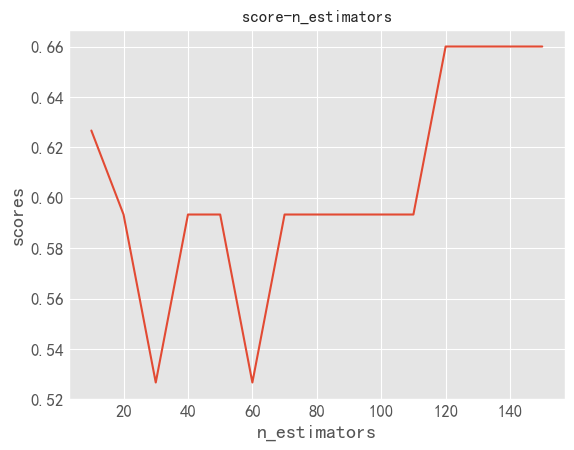
\includegraphics[width=0.7\textwidth]{6.png} %插入图片,[]中设置图片大小,{}中是图片文件名
	\caption{决策树数量图} %最终文档中希望显示的图片标题
	\label{Fig.main7} %用于文内引用的标签
\end{figure}

由图6知,在决策树的数量为120时,模型得分已经达到峰值,此时可以确定决策树的数量最佳值为120。

利用此模型对纹饰、类型、颜色三个特征进行特征重要性计算,结果如下:

\begin{table}[H]
	\centering
	\begin{tabular}{c c c c c c c} 
        \toprule[1.5pt]
		变量 & 纹饰A & 纹饰B & 纹饰C & 高钾类型 & 铅钡类型 & 颜色 \\ 
	    \midrule[1pt]
		评分 & 0.0963 & 0.1014 & 0.0518 & 0.1708 & 0.1809 & 0.3987 \\
        \toprule[1.5pt]
	\end{tabular}
\caption{评分表}
\end{table}



由表1可以看出玻璃纹饰C,纹饰A,纹饰B的评分低,玻璃类型次之,玻璃颜色最大;故本问得出玻璃颜色与玻璃表面风化的关系最强,玻璃的类型次之,而玻璃纹饰与玻璃表面风化关系最弱。结果表示与单个变量重要性之间有所差别,下面进一步说明树模型结果的可靠性以及两种结果差别的原因。

\subsubsection{模型评价}

树模型在本问中能够得到的结果是否可信,需要进一步对模型进行评价。通常是主要通过热力图和ROC图进行判断,同时利用准确率(0.78),精确率,召回率,F1分数,支持率来综合判断模型。根据以上得到的模型参数利用python对模型进行调参后形成新的模型,得到热力图并绘制了ROC曲线测试模型,如下图所示:


\begin{figure}[H] 
	\centering %图片居中
	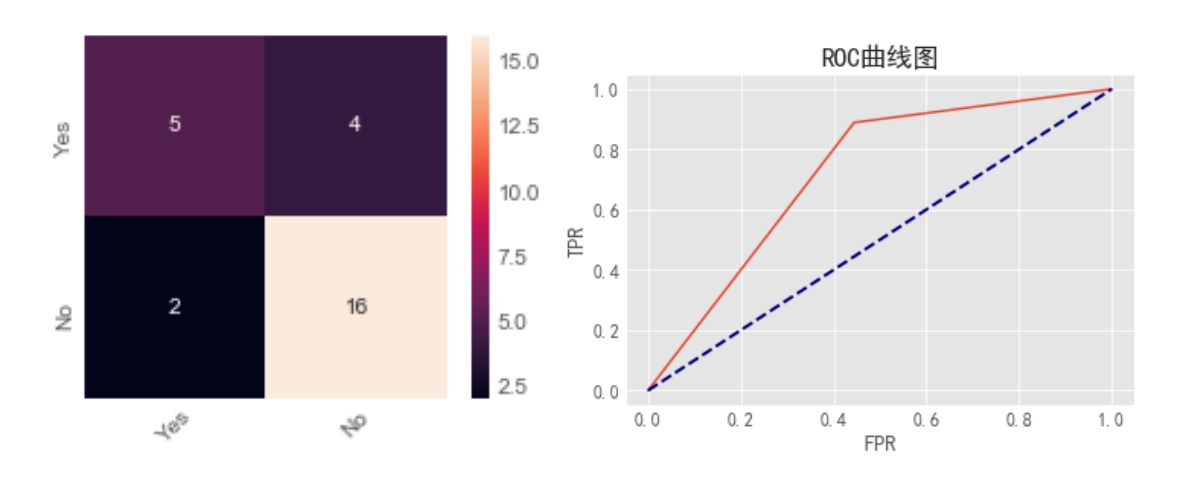
\includegraphics[width=0.7\textwidth]{7.png} %插入图片,[]中设置图片大小,{}中是图片文件名
	\caption{分类结果混淆矩阵热力图} %最终文档中希望显示的图片标题
	\label{Fig.main8} %用于文内引用的标签
\end{figure}

由图7可知,通过热力图知该模型中正确判断未风化的比例占8/9,正确判断风化的比列占5/9;ROC曲线图中可看出此模型的分类器性能极佳,由此认为这个模型可以用来分析批判纹饰、类型、颜色及风化表面之间关系。

对于分类模型的评价还有很多基于混淆矩阵的方法,结合对测试集的预测结果和测试集自身标签、通过计算得到模型的精确度得到如下指标:
\begin{table}[H]
	\centering
	\begin{tabular}{c c c c c} 
		\toprule[1.5pt]
			 & 精确度 & 召回率 & F1分数 & 支持率 \\ 
		\midrule[1pt]
		铅钡 &	0.71 &	0.56 &	0.63 &	9 \\
		高钾 & 	0.80 &	0.89 &	0.84 &	18 \\
		加权平均 &	0.77 &	0.78 &	0.77 &	27 \\
		\toprule[1.5pt]
	\end{tabular}
	\caption{评分数据表}
\end{table}


由表2可知,利用该模型对玻璃类型中高钾和铅钡检验得到的精确度均大于百分之七十,召回率均大于百分之五十,其中高钾类召回率高达百分之八十九,由此可知该模型极为可信,说明该模型对于三种特征的特征重要性评分具有可信度。对于上面结果的不完全相同,可能由于单变量特征重要性没有量化评判标准,导致结果有部分不同,但颜色特征关联最大的特征是确定的,下面对于不同特征重要性进行验证。


\subsubsection{互信息验证}

寻找特征与标签的关系的手段并不是单一的,针对本题数据的具体情况,由于特征和标签均为分类型变量,本文也通过计算互信息以衡量特征与标签间的独立性来验证此题结果。

利用互信息计算风化表面与纹饰,类型,颜色的互信息进一步验证每种关联性的科学性,公式如下:

\begin{equation}
    {{I}_{i}}\left( {{x}_{i}};{{x}_{4}} \right)=\displaystyle\sum\nolimits_{{{x}_{i}},{{x}_{4}}}{p({{x}_{i}},{{x}_{4}})}\log \frac{p({{x}_{i}},{{x}_{4}})}{p({{x}_{i}})p({{x}_{4}})}
\end{equation}

得到互信息表如下: 

\begin{table}[H]
	\centering
	\begin{tabular}{c c c c c} 
	    \toprule[1.5pt]
		& 纹饰 &	类型 &	颜色 &	表面风化情况 \\ 
		\midrule[1pt]
		纹饰 & 	0.943384 &	0.138290 & 	0.383740 &	0.061379 \\
		\hline
		类型 &	0.138290 &	0.619376 &	0.230124 &	0.059385 \\
		\hline
		颜色 &	0.383740 &	0.230124 &	1.609943 &	0.077623 \\
		\hline
		表面风化情况 &	0.061379 &	0.059385 &	0.077623 &	0.678209 \\
	    \toprule[1.5pt]
	\end{tabular}
\caption{互信息表}
\end{table}


由表3知由于纹饰和类型与玻璃表面风化情况的相关性值相差不大(约为0.02),可忽略不计,造成在多个变量共同作用时,类型的占比增大,因此类型的评分增大;而颜色与表面风化情况的相关性评分比其余两个都强,故认为颜色与玻璃文物表面风化有很大联系;此结果与上述模型结果显示一致,由此认为树模型是一个较好的模型且适用于玻璃风化与不同特征重要性评价。

\subsection{分析玻璃化学含量描述性模型}

要结合玻璃类型分析文物样本有无风化化学成分含量的统计规律,本问分别对高钾类和铅钡类玻璃风化情况与各化学成分关系进行数据可视化分析以及显著性检验来探究风化情况不同时化学成分的差异。

\subsubsection{数据可视化初探风化情况与化学成分浅层关系}

用Python读取由附件表2手动处理后的有效数据并提取出高钾类玻璃的数据。利用matplotlib得到高钾类玻璃风化与各化学成分关系的直方图,如下所示:

\begin{figure}[H] 
	\centering %图片居中
	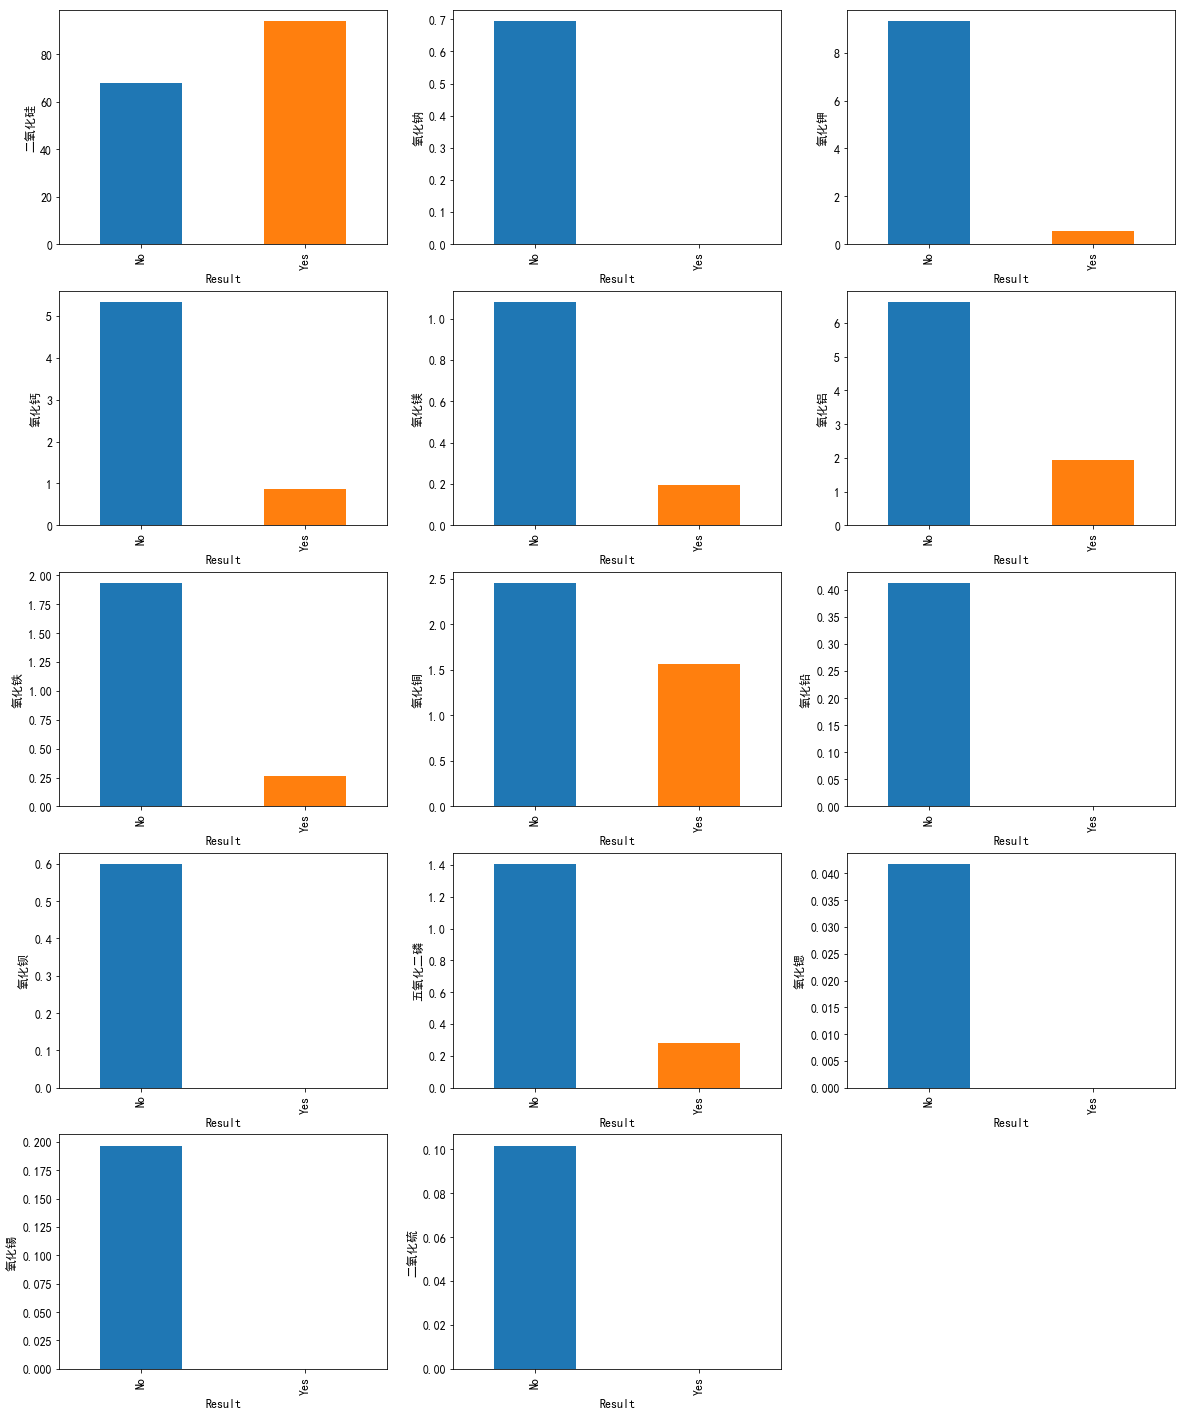
\includegraphics[width=0.7\textwidth]{8.png} %插入图片,[]中设置图片大小,{}中是图片文件名
	\caption{高钾类玻璃风化与各化学成分关系直方图} %最终文档中希望显示的图片标题
	\label{Fig.main9} %用于文内引用的标签
\end{figure}


由图8可知高钾玻璃中含氧化钠、氧化铅、氧化钡、氧化锶、氧化锡以及二氧化硫等化学分成表面未风化的均值较高,而表面风化的均值为0;氧化钾、氧化钙、氧化镁、氧化铝、氧化铁、五氧化二磷等化学分成表面未风化的均值均远大于表面风化的均值;由此可知风化的玻璃中含有氧化钠、氧化铅、氧化钡、氧化锶、氧化锡以及二氧化硫等化学成分含量较少,而含氧化钾、氧化钙、氧化镁、氧化铝、氧化铁、五氧化二磷等成分相对于多一些;另外,由于二氧化硅为玻璃制作的主要原材料,在化学成分中分布很广,在分析与玻璃风化是否有联系的结果并不是很明显。故玻璃风化联系最紧密的化学成分是氧化铜,所有化学成分与玻璃未风化联系都紧密。

同理本文可得到铅钡类玻璃风化与各化学成分关系的直方图如下:


\begin{figure}[H] 
	\centering %图片居中
	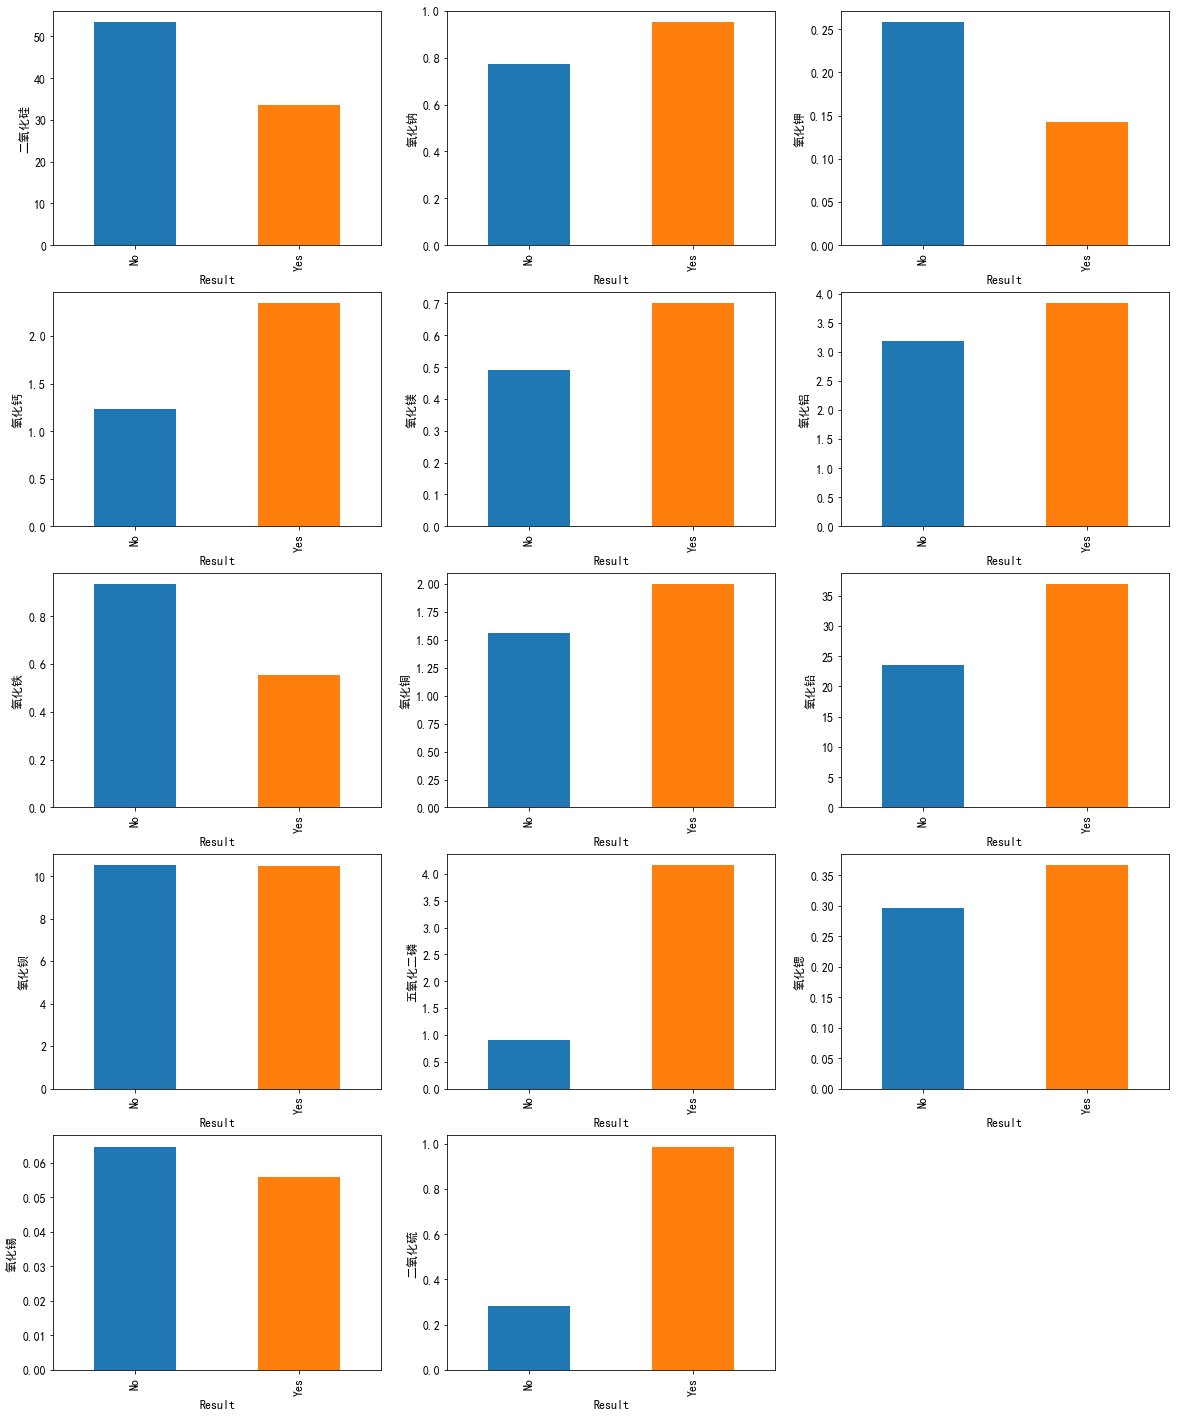
\includegraphics[width=0.7\textwidth]{9.png} %插入图片,[]中设置图片大小,{}中是图片文件名
	\caption{铅钡类玻璃风化与各化学成分关系直方图} %最终文档中希望显示的图片标题
	\label{Fig.main10} %用于文内引用的标签
\end{figure}

由图9知对于铅钡类玻璃中二氧化硫与五氧化二磷两种化学成分表面风化均值占比远高于表面未风化均值;而二氧化硅、氧化钾、氧化镁三个化学成分中玻璃表面风化均值低于表面未风化的均值;其余化学成分与表面是否风化占比相差不大。故二氧化硫与五氧化二磷两种化学成分绝大多数被风化,其余化学成分风化与被风化的程度相差不大。

\subsubsection{显著性检验考察风化情况下各化学成分差异性}

依据以上得到的数据可视化图,为了检验风化前后化学成分是否有明显变化,分别对高钾玻璃和铅钡玻璃风化前后对应的化学成分进行显著性检验。首先进行正态性检验得到下表:

\begin{table}[H]
	\centering
	\begin{tabular}{c c c c c c c} 
	    \toprule[1.5pt]    
		二氧化硅 & 氧化钠 & 氧化钾 & 	… & 氧化锶 & 氧化锡 & 二氧化硫 \\
		\midrule[1pt]
		0 &	0.002680 &	0 &	… &	0.002680 &	0.002680 &	0.002680 \\
	    \toprule[1.5pt]
	\end{tabular}
\caption{高钾玻璃化学成分正态检验部分表}
\end{table}

由上表发现化学成分均未通过正态性检验。

假设风化前后的化学成分有显著性差异,对于通过正态性检验的成分进行配对样本t检验,结果如下:

\[p\_value = 0.10991037\]

故拒绝原假设,氧化铜在高钾玻璃风化前后不具有显著差异。

假设风化前后的化学成分有显著性差异,对于未通过正态性检验的成分进行配对Milcoxon检验,结果如下:

\begin{table}[H]
	\centering
	\begin{tabular}{c c c c c c c} 
		\toprule[1.5pt]
		二氧化硅 &	氧化钠 & 氧化钾 &	… &	氧化锶 & 氧化锡 &	二氧化硫 \\
		\midrule[1pt]
		0.002526 &	0.181449 &	0.003263 &	… &	0.5 & 1 & 0.181449 \\
		\toprule[1.5pt]
	\end{tabular}
\caption{配对检验表}
\end{table}

氧化钠、氧化铜、氧化钡、氧化锶、二氧化硫五种成分拒绝原假设,在高钾玻璃风化前后不具有显著性差异;其他成分接受原假设,在风化前后具有显著性差异。
同理可得铅钡玻璃化学成分正态性检验表:

\begin{table}[H]
	\centering
	\begin{tabular}{c c c c c c c} 
		\toprule[1.5pt]
		二氧化硅 & 氧化钠 & 氧化钾 & … & 氧化锶 & 氧化锡 & 二氧化硫 \\
		\midrule[1pt]
		0.279 & 0.001*** &	0.005*** &	… &	0.585 &	0.000*** & 0.000*** \\
		\toprule[1.5pt]
	\end{tabular}
\caption{铅钡玻璃化学成分正态检验部分表}
\end{table}

由上表得:化学成分氧化钠、氧化钾、氧化铁、氧化锡、二氧化硫未通过正态性检验,化学成分二氧化硅、氧化钙、氧化镁、氧化铝、氧化铜、氧化铅、氧化钡、五氧化二磷、氧化锶通过正态性检验。

假设风化前后的化学成分有显著性差异,对于未通过正态性检验的成分进行配对Milcoxon检验,结果如下:

\begin{table}[H]
	\centering
	\begin{tabular}{c c c c c c c} 
		\toprule[1.5pt]
		二氧化硅 &	氧化钠 & 氧化钾 &	… &	氧化锶 & 氧化锡 & 二氧化硫 \\
		\midrule[1pt]
		0.000*** & 0.273 & 0.894 & … & 0.217 & 0.001*** & 0.225 \\
		\toprule[1.5pt]
	\end{tabular}
\caption{配对检验表}
\end{table}

二氧化硅、氧化钙、氧化镁、氧化铝、氧化铜、氧化铅、氧化钡、五氧化二磷、氧化锶九种成分拒绝原假设,在铅钡玻璃风化前后不具有显著性差异;其余化学成分不拒绝原假设,其他成分接受原假设,在风化前后具有显著性差异。


\subsection{预测风化前的化学成分含量}

\subsubsection{高钾、铅钡玻璃风化前后数据分析}

把高钾和铅钡玻璃对表面是否风化的数据分别进行分析,得到部分结果如下表详情见附件。

\begin{table}[H]
	\centering
	\begin{tabular}{c c c c c c} 
        \toprule[1.5pt]
		 & 二氧化硅 & 氧化钠 & 氧化钡 & 二氧化硫	& 五氧化二磷 \\
        \midrule[1pt]
		数量 & 12.00000 & 12.00000 & 12.00000 & 12.00000 & 12.00000 \\
		总和 & 67.984167 & 0.695000 & 0.598333 & 0.101667 & 1.402500 \\
		占比 & 8.755099 &	1.286917 & 0.982102 & 0.185513 & 1.433959 \\
		最小值	& 59.0100 & 0.0000 & 0.0000 & 0.0000 & 0.0000 \\
		$\frac{1}{4}$百分点 & 61.6775 & 0.0000 & 0.0000 & 0.0000 &	0.6900 \\
		$\frac{1}{2}$百分点 & 65.5300 & 0.0000 & 0.0000 & 0.0000 & 1.0200 \\
		$\frac{3}{4}$百分点 &  71.1675 & 0.5250 & 1.0725 &	0.0000 &	1.2925 \\
		最大值 & 87.050000 & 3.380000 & 2.860000 & 2.360000 & 4.500000 \\
		\toprule[1.5pt]
	\end{tabular}
\caption{高钾类玻璃风化前部分数据分析}
\end{table}

接下来对高钾玻璃风化前后数据进行可视化,得到以下可视化分布图:

\begin{figure}[H] 
	\centering %图片居中
	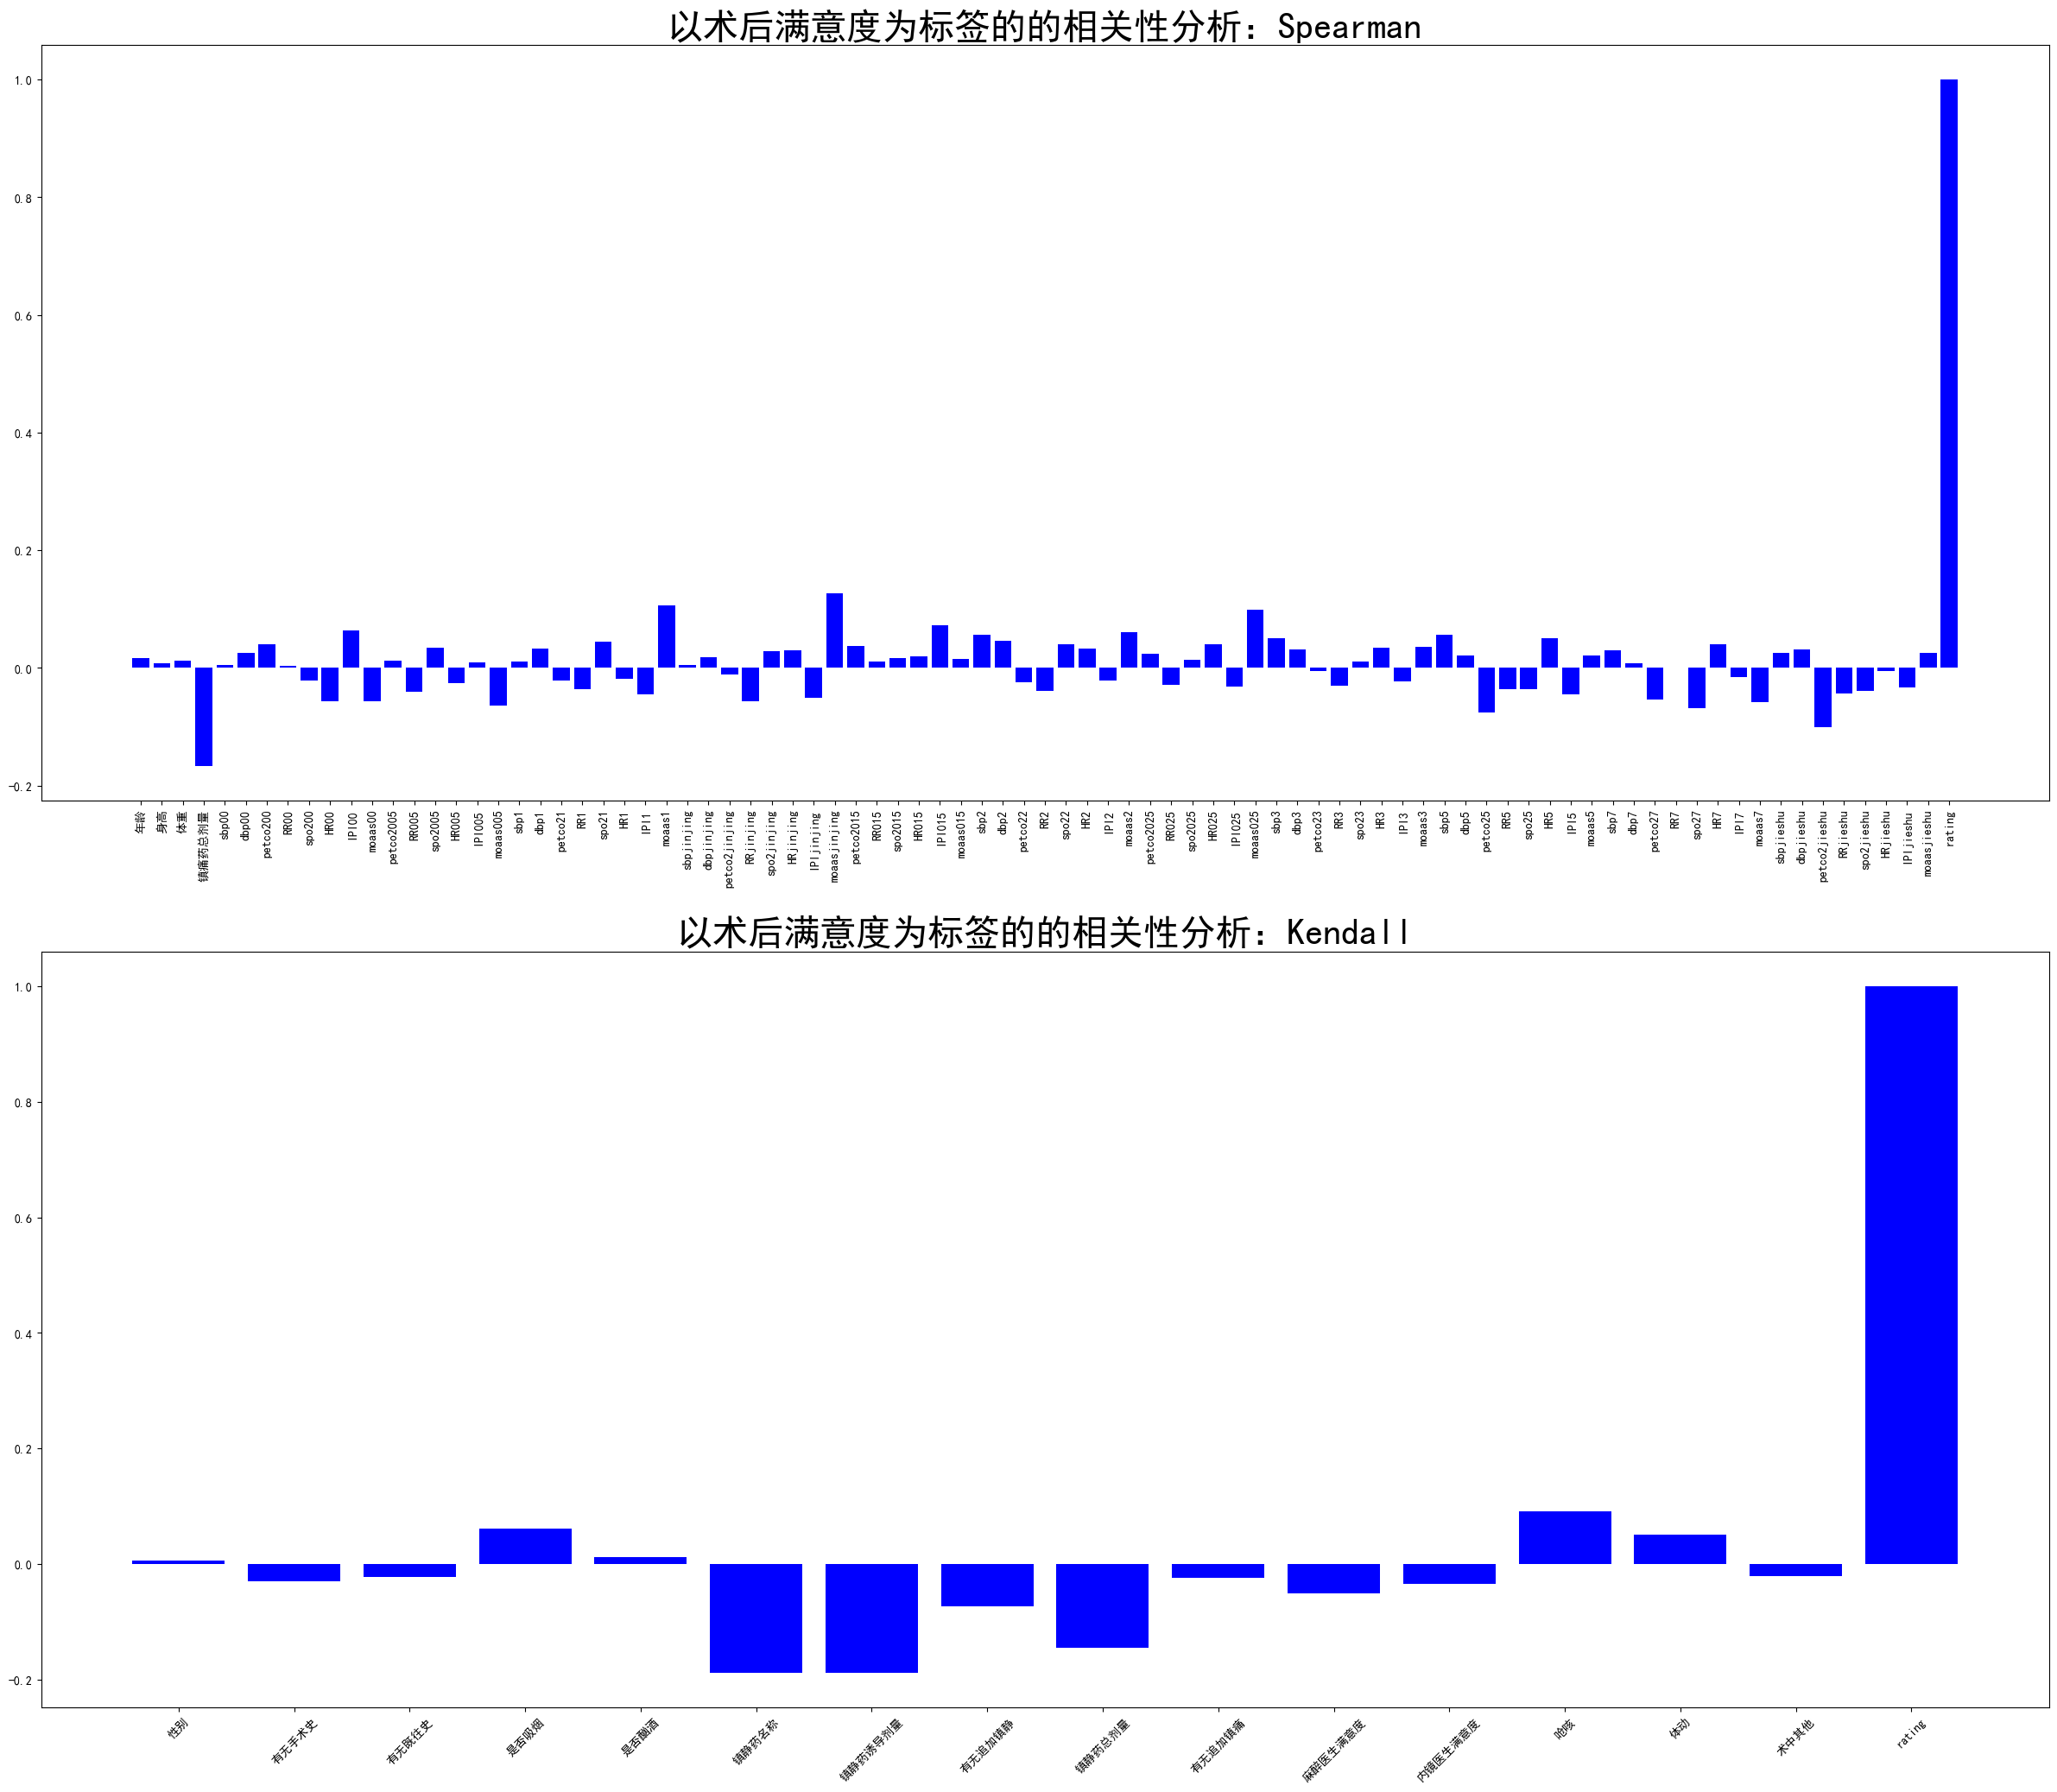
\includegraphics[width=0.7\textwidth]{10.png} %插入图片,[]中设置图片大小,{}中是图片文件名
	\caption{左图为高钾玻璃风化前各成分分布图;右图为高钾玻璃风化后各成分分布图} %最终文档中希望显示的图片标题
	\label{Fig.main11} %用于文内引用的标签
\end{figure}

调用Matplotlib的boxplot函数对高钾玻璃风化前后各特征的分布进行可视化,查看各特征离群值数量的多少。通过图10可以见高价玻璃风化前后各个化学成分的离群值较少,因此通过平均数可以反应数据各特征的一般水平。

\begin{figure}[H] 
	\centering %图片居中
	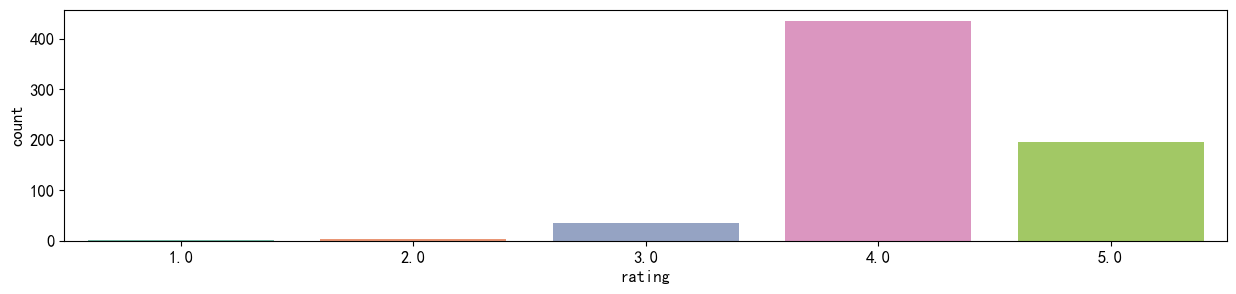
\includegraphics[width=0.7\textwidth]{11.png} %插入图片,[]中设置图片大小,{}中是图片文件名
	\caption{左图为铅钡玻璃风化前各成分分布图;右图为铅钡玻璃风化后各成分分布图} %最终文档中希望显示的图片标题
	\label{Fig.main12} %用于文内引用的标签
\end{figure}

通过图11可得铅钡玻璃风化前后各个化学成分的离群值依然较少,因此可以通过平均数来反映数据各个特征的一般水平。

\subsubsection{求取平均值、预测风化前化学成分}

由上把高钾和铅钡玻璃数据分析后可得数据异常值较少,为寻找一个风化前后具有代表性的数据,本问对两种玻璃风化前后的数据分别求平均值,具体方法如下:

1. 根据公式

\begin{equation}
    \overline{{{y}_{ijz}}}=\frac{\sum{{{y}_{ijz}}}}{{{n}_{ijz}}}.
\end{equation}

可分别求出高钾玻璃和铅钡玻璃风化前后每种化学成分的平均值。

2. 对风化后数据异常值进行检验,发现没有异常值,根据得到的风化前后的数据平均值求出对应化学成分的平均含量比率作为该化学含量的一般比率。设$H_j$为第$j$类化学物质的比例系数,利用公式

\begin{equation}
    {{H}_{ij}}=\frac{\overline{{{y}_{iy1}}}}{\overline{{{y}_{iy2}}}}.
\end{equation}

分别得到高钾和铅钡玻璃风化前后各成分比例系数部份表如下,具体详情见附件:


\begin{table}[H]
	\centering
	\begin{tabular}{c c c} 
		\toprule[1.5pt]
		成分类型 & 高钾玻璃风化前后含量比值 & 铅钡玻璃风化前后含量比值 \\
		\midrule[1pt]
		二氧化硅 & 0.723518 & 2.145246 \\
		五氧化二磷 & 5.008929 & 0.171270 \\
		氧化钾 & 6.129310 & 1.936599 \\
		氧化钙 & 5.487288 & 0.456906 \\
		氧化镁	& 3.430052 & 0.757396 \\
		氧化铝	& 7.289308 & 7 1.075628 \\
		\toprule[1.5pt]
	\end{tabular}
\caption{风化前后比例系数表}
\end{table}



最后再通过公式

\begin{equation}
    y_{iy1}^{'}={{H}_{ij}}\cdot y_{iy2}^{'}.
\end{equation}

求出风化后的玻璃对应的风化前的化学物质含量,得到对应的部分结果如下表所示,详情见附件:

\begin{table}[H]
	\centering
    \begin{tabular}{c c c c c c} 
        \toprule[1.5pt]
        样本检测位点成分 &	二氧化硅 &	氧化钠 & 	\dots &	氧化锡 &	二氧化硫 \\
        \midrule[1pt]
        01 &	77.82951415 &	0 &	\dots &	0 &	0 \\
        02 &	67.01947595 &	0.695 &	\dots &	0.196666667 &	0.101666667 \\
        03 &	43.20524848 &	0 &	\dots &	0 &	0.531689189 \\
        \dots &	\dots &	\dots &	\dots &	\dots &	\dots \\
        31 &	54.5321458 &	0 &	\dots &	0 &	0 \\
        32 &	65.19401695 &	0 &	\dots &	0 &	0 \\
        \toprule[1.5pt]
    \end{tabular}
    \caption{风化前化学成分含量部分}
\end{table} 